\documentclass[t]{beamer}

% Load general definitions
% Preamble file - general definitions, package loading, etc.

%=================================
% Load packages
\usepackage{amssymb,amsmath}
\usepackage{graphicx}
\usepackage{url}
\usepackage{tikz}
\usetikzlibrary{mindmap,trees,arrows}
\usepackage{fancyvrb}
\usepackage[portuguese]{babel} 
\usepackage[utf8]{inputenc}
\usepackage{subfigure}
\usepackage{times}
\usepackage[T1]{fontenc}
\usepackage{cancel}
\usepackage{color}
\usepackage{listings}
\usepackage[document]{ragged2e}

%=================================
% Set mode
\mode<presentation>
{
	\usetheme{Madrid}
	\usecolortheme{structure}
	\useoutertheme{infolines}
	\setbeamercovered{invisible}
}

% Get rid of nav bar
\beamertemplatenavigationsymbolsempty

% Insert frame number at bottom of the page.
\usefoottemplate{\hfil\tiny{\color{black!90}\insertframenumber}} 

%=================================
% Define new commands

\newcommand\Real{{\mathbb{R}}}
%\newcommand{\vi}{\vspace{0.6\baselineskip}}
%\newcommand{\goodgap}{\hspace{\subfigtopskip}\hspace{\subfigbottomskip}}


% Equation environments
\newcommand{\beq}{\begin{equation}}
\newcommand{\eq}{\end{equation}}
\newcommand{\beqs}{\begin{equation*}}
\newcommand{\eqs}{\end{equation*}}
\newcommand{\beqn}{\begin{eqnarray}}
\newcommand{\eqn}{\end{eqnarray}}
% Bold variables
\newcommand{\mbf}[1]{\ensuremath{\mathbf{#1}}}
% Itemization
\newcommand{\bitem}{\begin{itemize}}
\newcommand{\eitem}{\end{itemize}}
\newcommand{\spitem}{\vskip 1em\item}
\newcommand{\bitems}{\begin{itemize}\item}
\newcommand{\benums}{\begin{enumerate}\item}
\newcommand{\eenum}{\end{enumerate}}
% color blocks
\newenvironment{colorblock}[2]{%
\setbeamercolor{block title}{#2}
\begin{block}{#1}}{\end{block}}
% Vertical spacing
\newcommand{\vone}{\vskip 1em}
\newcommand{\vhalf}{\vskip .5em}
% Frame environments
\newenvironment{ftst}[3][t]{%
\begin{frame}{environment=ftst,#1}
\frametitle{#2}
\framesubtitle{#3}}{\end{frame}}
\newenvironment{ftstf}[2]{
\begin{frame}[fragile,environment=ftstf]
\frametitle{#1}
\framesubtitle{#2}}{\end{frame}}
% colors
\definecolor{MyGray}{rgb}{0.5,0.5,0.5}
\definecolor{MyDBGray}{rgb}{0.1,0.1,0.4}
\definecolor{darkgreen}{rgb}{0,0.4,0}
\definecolor{black}{rgb}{0,0,0}
\def\defn#1{{\color{red} #1}}
% Footnote
\renewcommand{\thefootnote}{\alph{footnote}}
% Relaxed footnotes
\newcommand{\lfr}[1]{\let\thefootnote\relax\footnote{\tiny #1}}
% Verbatim environment - using FANCYVRB package
\DefineVerbatimEnvironment%
{rcode}{Verbatim}
{fontsize=\scriptsize}
% Verbatim environment - using LISTINGS package
%\lstnewenvironment{rcode} {\lstset{	language = R,
%									basicstyle = \scriptsize\ttfamily,
%									showspaces = false,
%									showstringspaces = false,
%									showtabs = false,
%									keywordstyle = \color{black}\bfseries,
%									commentstyle = \color{darkgreen},
%									numbers = none,
%									otherkeywords={	<-,
%													ggplot,
%													geom_boxplot,
%													facet_grid,
%													shapiro.test,
%													fligner.test,
%													glht,
%													with},
%									deletekeywords={data,
%													model,
%													residuals,
%													c,
%													axis,
%													default,
%													labels,
%													qq.text}}}%
%{}

% Specific definitions
\title[]{Metodologia Científica}
\subtitle[]{Referências/Citações}
\author[]{Patrícia Lucas\\{\footnotesize }}
\institute{Bacharelado em Sistemas de Informação \\ IFNMG  - Campus Salinas}
\date{\scriptsize Salinas\\Junho 2021}

\begin{document}

% cover page
\setbeamertemplate{footline}{}
\begin{frame}

\begin{center}
\includegraphics[width=.15\textwidth]{}
\end{center}
  \titlepage
  \begin{tikzpicture}[remember picture,overlay]
  \node[anchor=south east,xshift=-5pt,yshift=5pt] at (current page.south east) {\tiny Versão 1.2021};
  \node[anchor=south west,yshift=0pt] at (current page.south west) {
\includegraphics[width=.25\textwidth]{Logos/salinas_horizontal_jpg.jpg}};
  \end{tikzpicture}  
\end{frame}

% Main slides

%=====

\begin{ftst}{O que são?}{Referências/Citações}
\justifying
\textbf{O que é uma referência bibliográfica?} referência é o conjunto padronizado de elementos descritivos, retirados de um documento que permite sua identificação individual.
\vone
\textbf{O que é uma citação?} É informar para o leitor qual a fonte de uma determinada informação que você está se referindo no texto. Isso pode ser quando você está discutindo ou resumindo uma teoria ou informação com suas próprias palavras, ou pode estar citando diretamente dessa fonte.

\end{ftst}

%=====

\begin{ftst}{Exemplo}{Referências/Citações}
\justifying
\vone
\textbf{Citação:} O método STN foi introduzido em \textbf{Song e Chissom (1993) }para lidar com o conhecimento vago e impreciso em dados de séries temporais.
\vone
\textbf{Referência:} Song, Qiang; Chissom, Brad S. Fuzzy time series and its models. Fuzzy sets and systems, vol. 54, number 3, pp. 269–277, 1993. URL: https://doi.org/10.1016/0165-0114(93)90372-O. Acesso em 25/07/2018.
\vone
\vone
\vone
\small
\textbf{OBS:} Um DOI, ou Digital Object Identifier, é uma sequência de números, letras e símbolos usados para identificar permanentemente um artigo ou documento e criar um link para ele na web.
\vone
Dica de ferramenta para encontrar o bibtex de um artigo usando o DOI: \href{https://www.doi2bib.org/}{\textcolor{blue}{doi2bib.}}
\end{ftst}

%=====

\begin{ftst}{2 regras importantes}{Referências/Citações}
\justifying
\vone
\begin{itemize}
    \item[1.] usar referências \textbf{publicadas} e que sejam \textbf{significativas}. 
    \item[2.] garantir que todas as referências citadas no texto sejam realmente listadas na literatura citada e que todas as referências listadas na literatura citada sejam realmente citadas em algum lugar do texto.
\end{itemize}

\end{ftst}

%=====

\begin{ftst}{Significância das referências}{Referências/Citações}
\begin{table}[]
\centering
\scriptsize
\begin{tabular}{|c|l|}
\hline
\textbf{\begin{tabular}[c]{@{}c@{}}Tese de \\ doutorado\end{tabular}} &
  \begin{tabular}[c]{@{}l@{}}- Obrigação de expandir o conhecimento científico.\\ - Análise rigorosa e arguição por banca examinadora (entre 4 \\ e 6 doutores) em sessão pública.\\ - Qualidade, publicação de artigo em periódico e defesa final.\end{tabular} \\ \hline
\textbf{\begin{tabular}[c]{@{}c@{}}Artigo em periódico \\ científico \\ Livros acadêmico\end{tabular}} &
  \begin{tabular}[c]{@{}l@{}}- Revisão rigorosa por pares (entre 3 e 5 doutores).\\ - Diversas rodadas de revisão.\end{tabular} \\ \hline
\textbf{\begin{tabular}[c]{@{}c@{}}Dissertação de \\ mestrado\end{tabular}} &
  \begin{tabular}[c]{@{}l@{}}- Análise rigorosa e arguição por banca examinadora (entre 3 e 4\\  doutores) em sessão pública.\\ - Qualidade, publicação de trabalho em congresso e defesa final.\end{tabular} \\ \hline
\textbf{\begin{tabular}[c]{@{}c@{}}Trabalho completo \\ em congresso\end{tabular}} &
  \begin{tabular}[c]{@{}l@{}}- Resultados preliminares de pesquisa.\\ - Revisão por pares (2 revisores).\\ - Apresentação e arguição.\end{tabular} \\ \hline
\textbf{\begin{tabular}[c]{@{}c@{}}Monografia\\ Relatório técnico\end{tabular}} &
  \begin{tabular}[c]{@{}l@{}}- Relato de caso com aplicações técnicas.\\ - Análise não tão rigorosa, arguição por banca examinadora.\end{tabular} \\ \hline
\textbf{\begin{tabular}[c]{@{}c@{}}Resumo em \\ congresso\end{tabular}} &
  \begin{tabular}[c]{@{}l@{}}- Resultados preliminares de pesquisa.\\ - Revisão por pares (2 revisores).\end{tabular} \\ \hline
\end{tabular}
\end{table}

\end{ftst}

%=====

\begin{ftst}{Referências}{Referências/Citações}
\begin{figure}
    \centering
    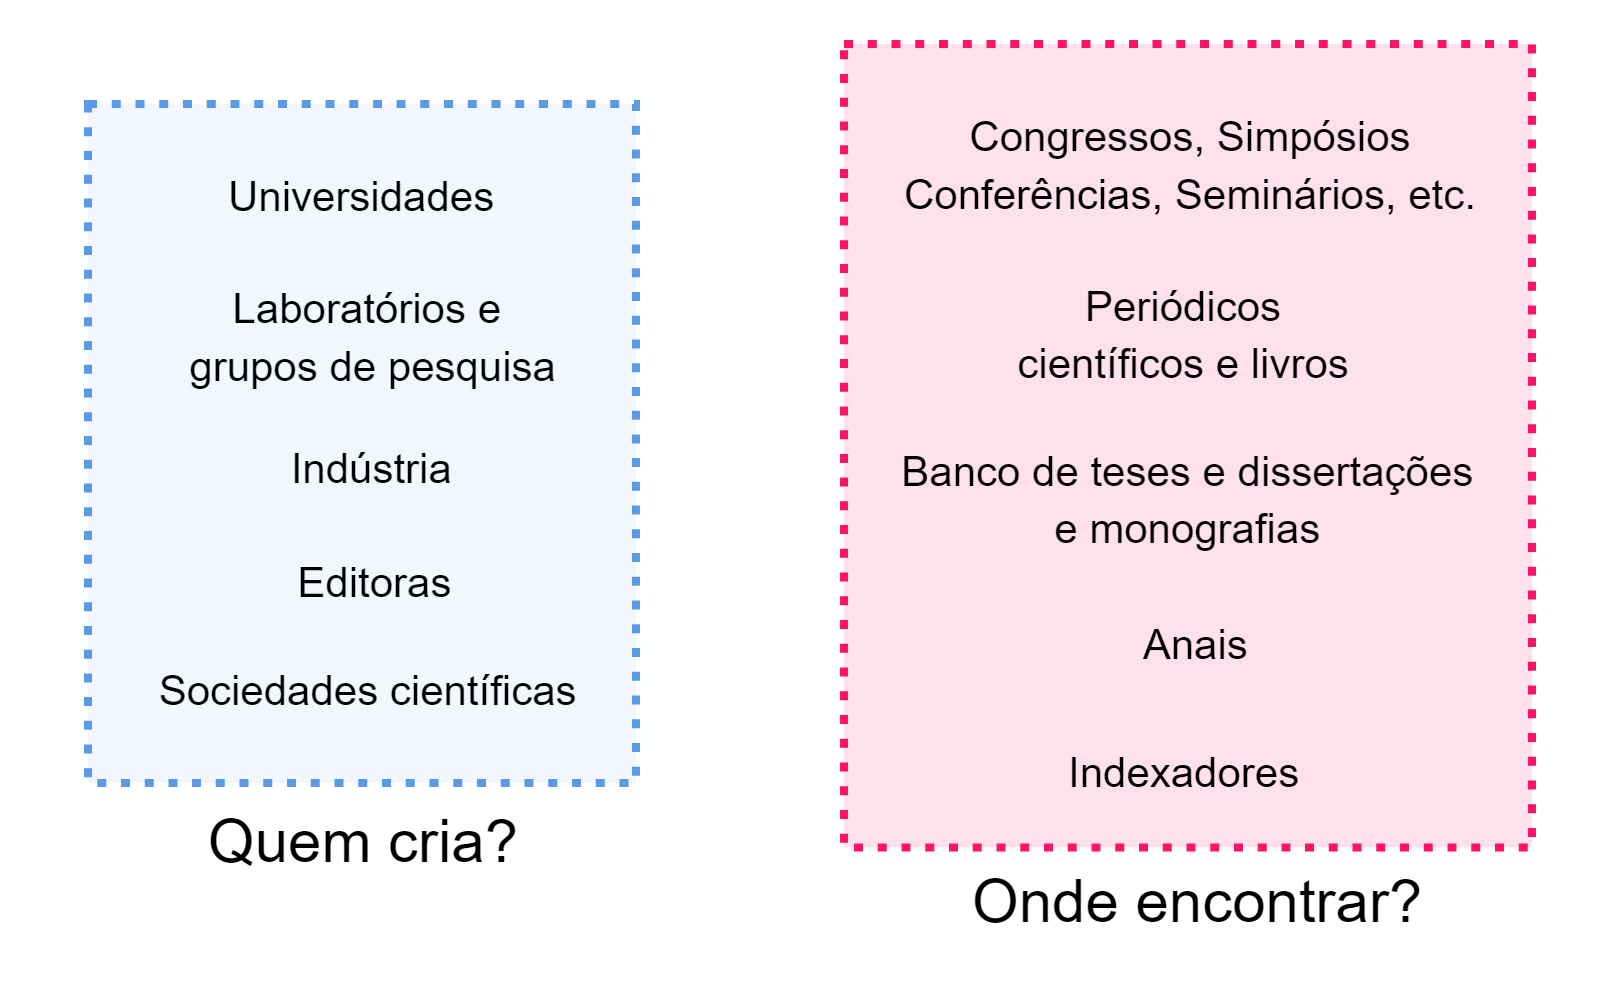
\includegraphics[scale=0.2]{Figuras/referecias_quemcria.png}
\end{figure}

\end{ftst}

%=====


\begin{ftst}{Busca bibliográfica}{Referências/Citações}
\justifying
Sugestão de passo a passo:
\begin{enumerate}
    \item Procure por palavras chave (poucas!).

    \item Selecione artigos de maior qualidade (veículo, nº de citações, tipo de pesquisa, etc.).

    \item Escolha a idade do artigo.

    \item Leia o resumo e escolha os mais relevantes.
    \item Para um artigo X escolhido:
    \begin{enumerate}
        \item As referências usadas nesse artigo podem ser úteis.
        \item Os artigos que citam X também podem ser úteis.
        \item Artigos relacionados: são "parecidos com X" e podem ser úteis para encontrar outras famílias de artigos.
    \end{enumerate}
\end{enumerate}
\vone
\small
\textbf{Ferramentas de busca: \href{https://www-periodicos-capes-gov-br.ezl.periodicos.capes.gov.br/index.php?}{\textcolor{blue}{Site de periódicos da CAPES}}, \href{https://scholar.google.com.br/?hl=pt}{\textcolor{blue}{Google Acadêmico}}, \href{https://www.mendeley.com/}{\textcolor{blue}{Mendeley}}, \href{https://dblp.org/}{\textcolor{blue}{dblp}}, etc.}

\end{ftst}


%=====

\begin{ftst}{Tipos de citação}{Referências/Citações}
\justifying

\begin{itemize}
    \item Citação Direta: pode ser definida como a transcrição de um trecho completo da obra que está sendo consultada, ou seja, é a transcrição mais literal possível que o estudante utiliza e essa exige uma margem para ser usada no trabalho acadêmico em especial. \textcolor{red}{Não são usuais na área da Computação!}
    \vone
    \item Citação Indireta: pode ser chamada também de paráfrase, essa é usada quando o estudante faz uma conexão do texto com outro autor, ou seja, faz o uso, porém com suas palavras.
    \vone
    \item Citação de Citação: quer dizer que seria uma citação usada de uma citação usada por outro autor(a). \textcolor{red}{Não use!}
\end{itemize}
\end{ftst}

%=====

\begin{ftst}{Estilos}{Referências/Citações}
\justifying
\begin{itemize}
    \item \textbf{Formato Harvard:} \href{https://www.mendeley.com/guides/harvard-citation-guide}{\textcolor{blue}{guia completo aqui}.}
    \vone
    \item \textbf{Formato Vancouver:} \href{https://guides.lib.monash.edu/citing-referencing/vancouver}{\textcolor{blue}{guia completo aqui}.}
    \vone
    \item \textbf{Formato IEEE:} \href{https://journals.ieeeauthorcenter.ieee.org/your-role-in-article-production/ieee-editorial-style-manual/}{\textcolor{blue}{guia completo aqui}.}
    \vone
    \item \textbf{Formato ABNT:} \href{https://www.ufpe.br/documents/40070/1837975/ABNT+NBR+6023+2018+\%281\%29.pdf/3021f721-5be8-4e6d-951b-fa354dc490ed}{\textcolor{blue}{NBR 6023}.}
    \href{http://www2.uesb.br/biblioteca/wp-content/uploads/2016/05/NBR-10520-CITA\%C3\%87\%C3\%95ES.pdf}{\textcolor{blue}{NBR 10520}.}
\end{itemize}

\end{ftst}




\end{document}